\newcommand{\componentA}{0.88}
\newcommand{\componentB}{0.96}
\newcommand{\componentC}{0.997}

\definecolor{motivation}{rgb}{\componentA, \componentB, \componentC}
\definecolor{building}{rgb}{  \componentB, \componentC, \componentA}
\definecolor{basics}{rgb}{    \componentB, \componentA, \componentC}
\definecolor{lists}{rgb}{     \componentA, \componentC, \componentB}
\definecolor{errors}{rgb}{    \componentC, \componentA, \componentB}
\definecolor{templates}{rgb}{ \componentC, \componentB, \componentA}
\definecolor{exercises}{rgb}{ \componentA, \componentB, \componentC}

\newcommand{\bgcolor}{Purple} % this should be renewed below

%%%%%%%%%%%%%%%%%%%%%%%%%%%%%%%%%%%%%%%%%%%%%%%%%%%%%%%%%%%%%%%
%%%%%%%%%%%%%%%%%%%%%%%%%%%%%%%%%%%%%%%%%%%%%%%%%%%% Motivation

% background color pre
{
\setbeamercolor{background canvas}{bg=motivation}
\renewcommand{\bgcolor}{motivation}

\section{Motivation}
\begin{frame}
  \vspace{25mm}
  \begin{center}
    \Huge{Part 1:\\Motivation}
  \end{center}
\end{frame}

\subsection{Observations}
\begin{frame}[fragile]
  \frametitle{Observations}
  \vspace{3mm}
  WYSIWYG editors provide plenty of distractions that compete for your attention.
  \begin{itemize}
    \item That attention is key to good writing.
    \item These distractions slows down the writing process.
  \end{itemize}
  
  \vspace{5mm}
  WYSIWYG editors provide little help managing references of any kind.
  
  \vspace{5mm}
  WYSIWYG editors generally encourage bitmapped graphics.
  
  \vspace{5mm}
  WYSIWYG editors tends to result little consistency in the resulting documents.
  
  \vspace{5mm}
  The formats employed by WISIWYG editors are usually horrible in terms of version control.
  
  \vspace{5mm}
  WISIWYG editors are usually horrible for collaborative editing.
\end{frame}

\subsection{Why \LaTeX?}
\begin{frame}[fragile]
  \frametitle{Why \LaTeX? [1/2]}
  \vspace{3mm}
  \LaTeX\ is a programming language saved in clear text files using markup code.
  \begin{itemize}
    \item This makes it suitable for version control.
    \item Version control is a form of collaborative editing.
    \item Web-based editors (like overleaf) exists and work fairly well.
  \end{itemize}
  
  \vspace{5mm}
  \LaTeX\ (mostly) decouples structure and presentation.
  \begin{itemize}
    \item This results in highly consistent layouts.
    \item When writing, you can focus on the structure.
    \item If you wish to, you can \textsl{choose} to dig into the nitty gritty details.
    \item But there is rarely a need: Most templates make the result look great without intervention.
  \end{itemize}
\end{frame}
\begin{frame}[fragile]
  \frametitle{Why \LaTeX? [2/2]}
  \vspace{2mm}
  \LaTeX\ is a highly extendable and mature system with lots of tools designed for technical documents.
  \begin{itemize}
    \item Working with a bibliography is trivial.
    \item Working with an index is trivial.
    \item Working with floats (like figures and tables) is trivial.
    \item Working with equations is simple.
    \item References to any of these \textsl{just work}.
  \end{itemize}
  
  \vspace{4mm}
  \LaTeX\ is a professional typesetting system and thus vector based.
  \begin{itemize}
    \item It is trivial to include vector graphics.
    \item But it is also trivial to include bitmapped graphics.
  \end{itemize}
  
  \vspace{4mm}
  \textbf{Note:} This essentially mitigates the observations.
\end{frame}

\subsection{What is \LaTeX?}
\begin{frame}[fragile]
  \frametitle{What is \LaTeX?}
  \vspace{3mm}
  \LaTeX\ is a programming language that, when evaluated, produces a PDF file.
  
  \vspace{5mm}
  It relies heavily on the concept of macro expansion.
  
  \vspace{5mm}
  \LaTeX\ is extended through packages. Currently there are 6000+ such packages on CTAN: \url{https://ctan.org}
\end{frame}

\subsection{Styles}
\begin{frame}[fragile]
  \frametitle{What is \LaTeX? \subpart{Styles}}
  \vspace{3mm}
  In \LaTeX, contents and presentation are (mostly) separate.
  
  \vspace{5mm}
  During your day-to-day writing you care about structure: Sections, paragraphs, emphasis, listing \ldots
  
  \vspace{5mm}
  You don't care about how these are effectualized: Margins, fonts, colors, spacing, indents \ldots
  
  \vspace{5mm}
  These things are (generally speaking) covered by a \textsl{style}, and it typically does a very good job.
  
  \vspace{5mm}
  Should you not be happy with the styling rules defined in your style, then you can:
  \begin{enumerate}
    \item Pick another.
    \item Adjust it.
    \item Hardcode specifics.
  \end{enumerate}
\end{frame}

\subsection{When to Not \LaTeX?}
\begin{frame}[fragile]
  \frametitle{When to Not \LaTeX?}
  \vspace{3mm}
  \begin{itemize}
    \descitem{Note Taking} I find that \textsl{markdown} fulfills this role adequately, and is faster to write.
    \descitem{Audience Expectations} Often, your audience will expect a Word file, and then it just doesn't make sense.
    \descitem{Web} It it has to go on the web, something that was originally meant for HTML production is likely the way to go.
  \end{itemize}
\end{frame}

% background color post
}

%%%%%%%%%%%%%%%%%%%%%%%%%%%%%%%%%%%%%%%%%%%%%%%%%%%%%%%%%%%%%%%
%%%%%%%%%%%%%%%%%%%%%%%%%%%%%%%%%%%%%%%%%%%%%% Building the PDF

% background color pre
{
\setbeamercolor{background canvas}{bg=building}
\renewcommand{\bgcolor}{building}

\section{Building the PDF}
\begin{frame}
  \vspace{25mm}
  \begin{center}
    \Huge{Part 2:\\Building the PDF}
  \end{center}
\end{frame}

\subsection{Engines}
\begin{frame}[fragile]
  \frametitle{Engines}
  \vspace{2mm}
  In order to compile a \LaTeX\ document into PDF you need a \LaTeX\ engine.
  
  \vspace{4mm}
  Options:
  \begin{itemize}
    \descitem{pdflatex} The old engine that is fast but lacks native unicode and modern OpenType font support. These are not serious restrictions.
    \descitem{xelatex} A more modern version of \textdesc{pdflatex} that fixes its downsides. But on the flipside it is slower and has not been actively developed since 2017.
    \descitem{lualatex} The most modern engine is scriptable through Lua. It also fixes the issues with \textdesc{pdflatex} and is under active development. It is even slower though.
      \begin{itemize}
        \item This is the way to go for new projects.
        \item From this point on, we will assume \textdesc{lualatex}.
        \item Don't worry too much about the lack of speed. It is rare that it becomes an annoyance.
        \item While you can script it in Lua, the interactions with the \LaTeX\ macro system are complex. Personally, I have decided against it.
      \end{itemize}
  \end{itemize}
\end{frame}

\subsection{Distributions}
\begin{frame}[fragile]
  \frametitle{Distributions}
  \vspace{3mm}
  For you to work with \LaTeX, you will need:
  \begin{itemize}
    \item A number of appropriate fonts.
    \item A \LaTeX\ engine for compiling.
    \item A collection of packages with extensions.
    \item A number of other support programs.
  \end{itemize}
  
  \vspace{5mm}
  All of this combined is referred to as a \LaTeX\ distribution.
  
  \vspace{5mm}
  There exists a number of precompiled distributions:
  \begin{itemize}
    \descitem{\TeX\ Live} The typical distribution (Linux, Windows and OSX).
    \descitem{MiKTeX} If you are on Windows (but also works in Linux and OSX).
    \descitem{MacTeX} If you are on a Mac.
  \end{itemize}
\end{frame}

\subsection{Commandline}
\begin{frame}[fragile]
  \frametitle{Commandline}
  \vspace{3mm}
  Running the \LaTeX\ interpreter is done using the following command:
  \begin{minted}[breaklines]{shell-session}
lualatex document.tex
  \end{minted}
  or, if you are using \packagename{minted} for source code highlighting:
  \begin{minted}[breaklines]{shell-session}
lualatex -shell-escape document.tex
  \end{minted}
  
  \vspace{5mm}
  \textbf{Note:} When using references, you may have to run the command multiple times.
\end{frame}

\subsection{Overleaf}
\begin{frame}[fragile]
  \frametitle{Overleaf}
  \begin{tikzpicture}[remember picture,overlay]
    \node[anchor=south] () at ([yshift=-1.2cm]current page.south) {
      \only<1>{\includeBitmap{overleafmain.png}{14cm}}\only<2>{\includeBitmap{overleafdemo.png}{14cm}}
    };
  \end{tikzpicture}
\end{frame}

\subsubsection{Hosting Options}
\begin{frame}[fragile]
  \frametitle{Overleaf \subpart{Hosting Options}}
  \vspace{3mm}
  Cloud:
  \begin{itemize}
    \item Paid and free tier.
    \item Paid tier provices GIT support.
    \item Issues with uptime.
  \end{itemize}
  
  \vspace{5mm}
  Self-hosted:
  \begin{itemize}
    \item No GIT support.
    \item If all else fails, you can pull the data out yourself.
  \end{itemize}
\end{frame}

\subsection{Make}
\begin{frame}[fragile]
  \frametitle{Make}
  \vspace{-1mm}
  \inputminted[fontsize=\tiny]{make}{Makefile}
\end{frame}

\subsection{GIT}
\begin{frame}[fragile]
  \frametitle{GIT}
  \vspace{3mm}
  GIT is used for keeping tract of revisions of (primarily) human-readable files.
  
  \vspace{5mm}
  This is usually used for program code.
  
  \vspace{5mm}
  \LaTeX\ is a programming language, and when we execute \LaTeX\ code (through an interpreter) then we get a PDF file.
  
  \vspace{5mm}
  A GIT repository can easily contain both your program code and your report.
  
  \vspace{5mm}
  Typical structure:
  \begin{itemize}
    \item Program code in \textcolor{purple}{\texttt{/src}} of the repository.
    \item Report and presentation in \textcolor{purple}{\texttt{/doc}} of the repository.
    \item Figures shared between report an presentation in \textcolor{purple}{\texttt{/doc/figs}} of the repository.
  \end{itemize}
\end{frame}

% background color post
}

%%%%%%%%%%%%%%%%%%%%%%%%%%%%%%%%%%%%%%%%%%%%%%%%%%%%%%%%%%%%%%%
%%%%%%%%%%%%%%%%%%%%%%%%%%%%%%%%%%%%%%%%%%%%%%%%%%%%%%%% Basics

% background color pre
{
\setbeamercolor{background canvas}{bg=basics}
\renewcommand{\bgcolor}{basics}

\section{Basics}
\begin{frame}
  \vspace{25mm}
  \begin{center}
    \Huge{Part 3:\\Basics}
  \end{center}
\end{frame}

\subsection{Overall Structure}
\begin{frame}[fragile]
  \frametitle{Overall Structure}
  \begin{tikzpicture}[remember picture,overlay]
    \newcommand{\height}[0]{14mm}
    \newcommand{\width}[0]{3mm}
    
    \tikzstyle{segment} = [
      rectangle,
      rounded corners=1mm,
      anchor=north west,
      fill=purple,
      minimum height=\height,
      minimum width=\width,
    ]
    
    \coordinate (top) at ([yshift=34mm]current page.center);
    
    \node[anchor=north] (docclass) at (top) {\mintinline{latex}{\documentclass[a4paper, oneside]{memoir}}};
    
    \node[segment] (pa) at (docclass.south west) {};
    \node[anchor=west] () at (pa.east) {Preample};
    
    \node[anchor=north west] (begin) at (pa.south west) {\mintinline{latex}{\begin{document}}};
    
    \node[segment] (fm) at (begin.south west) {};
    \node[anchor=west] () at (fm.east) {Front Matter};
    
    \node[segment] (main) at (fm.south west) {};
    \node[anchor=west] () at (main.east) {Main Matter};
    
    \node[segment] (bm) at (main.south west) {};
    \node[anchor=west] () at (bm.east) {Back Matter};
    
    \node[anchor=north west] (end) at (bm.south west) {\mintinline{latex}{\end{document}}};
  \end{tikzpicture}
\end{frame}

\subsubsection{Packages}
\begin{frame}[fragile]
  \frametitle{Overall Structure \subpart{Packages}}
  \vspace{3mm}
  A package is a \LaTeX\ term for a file (or collection of files) that contain a set of macros (commands and environments) for dealing with a specialized topic.
  
  \vspace{5mm}
  The \packagename{dirtytalk} package gives access to the \commandname{\textbackslash say} command. This command takes one parameter and wraps it in the proper quotation marks, like \say{so}.
  
  \vspace{5mm}
  It can be included by putting the following in the \textcolor{purple}{\textsl{preample}}:
  \begin{minted}[breaklines]{latex}
\usepackage{dirtytalk}
  \end{minted}
  
  \vspace{5mm}
  This is a very simple package. Others -- like \TikZ\ and \packagename{minted} -- are much more extensive.
\end{frame}

\subsubsection{Language and Hyphenation}
\begin{frame}[fragile]
  \frametitle{Overall Structure \subpart{Language and Hyphenation}}
  \vspace{3mm}
  All of this goes into the \textcolor{purple}{\textsl{preample}}.
  
  \pause
  \vspace{5mm}
  Most parts of \LaTeX has multilingual support, selectable through the \packagename{babel} package:
  \begin{minted}[breaklines]{latex}
% use english text to ToC, sections, figures ...
\usepackage[english]{babel}
  \end{minted}
  
  \pause
  \vspace{5mm}
  Custom hyphenation rules can be added:
  \begin{minted}[breaklines]{latex}
\usepackage{hyphenat}
\hyphenation{al-go-rithm me-cha-nics}
  \end{minted}
\end{frame}

\subsubsection{File Inclusion}
\begin{frame}[fragile]
  \frametitle{Overall Structure \subpart{File Inclusion}}
  \vspace{3mm}
  As programmers, we usually have a good understanding of the problems that can stem from having all of our code in a single file.
  
  \vspace{5mm}
  In \LaTeX\ one can, in essence, include the contents of an other file like so:
  \begin{minted}[breaklines]{latex}
\input{filename.tex}
  \end{minted}
  
  \vspace{5mm}
  This is often used for top-level sections or figures.
  
  \pause
  \vspace{5mm}
  As programmers, we rarely have a good understanding of the problems of having all of our code split across an ocean of files.
  
  \pause
  \vspace{5mm}
  So, use with care.
\end{frame}

\subsubsection{Structure of Contents}
\begin{frame}[fragile]
  \frametitle{Overall Structure \subpart{Structure of Contents}}
  \vspace{3mm}
  The \textsl{main matter} is split into a section tree, with lists of paragraphs as leaves.
  
  \vspace{5mm}
  What is available to you depends on your \textsl{style}.
  
  \vspace{5mm}
  \begin{minted}[fontsize=\footnotesize,breaklines]{latex}
\part{Reasoning}
\section{Introduction}

paragraph 1

paragraph 2

\subsection{Problem}
\subsection{Approach}
\section{Analysis}
\subsection{Themes}
\subsubsection{Build Systems}
\subsubsection{Scripting}
\subsection{Sub-Conclusion}
  \end{minted}
\end{frame}

\subsection{Commands and Environments}
\begin{frame}[fragile]
  \frametitle{Commands and Environments}
  \vspace{3mm}
\end{frame}

\subsection{Spacing}
\begin{frame}[fragile]
  \frametitle{Spacing}
  \vspace{3mm}
  Whitespaces are treated the same way as in most other programming languages: Either there is at least one, or there is none. No need to worry about having two spaces instead of one.
  
  \vspace{5mm}
  Horizontal and vertical space can be added with the \commandname{\textbackslash hspace} and \commandname{\textbackslash vspace} commands. They both take one parameter; a distance.
  
  \vspace{5mm}
  \LaTeX\ will break the line as it tries to optimize the document layout (by minimizing \textsl{badness}) according to the rules of the style.
  
  \vspace{5mm}
  \textbf{Note:} This can make it hard to force a specific placement.
\end{frame}

\subsubsection{Horizontal Space}
\begin{frame}[fragile]
  \frametitle{Spacing \subpart{Horizontal Space}}
  \vspace{3mm}
  \begin{tikzpicture}[remember picture,overlay]
    \newcommand{\height}[0]{24mm}
    \newcommand{\dist}[0]{5mm}
    
    \tikzstyle{dedge} = [thick,->,>=stealth,draw=black]
    
    \node[rectangle,thick,anchor=east,draw,minimum height=\height] (code) at ([xshift=-\dist]current page.center) {
      \begin{minipage}{6cm}
        \begin{minted}[breaklines]{latex}
first\hspace{1cm}last
        \end{minted}
      \end{minipage}
    };
    
    \node[rectangle,thick,anchor=west,draw,minimum height=\height] (output) at ([xshift=\dist]current page.center) {
      \begin{minipage}{6cm}
        first\hspace{1cm}last
      \end{minipage}
    };
    
    \draw[dedge] (code)->(output);
  \end{tikzpicture}
\end{frame}

\subsubsection{Vertical Space}
\begin{frame}[fragile]
  \frametitle{Spacing \subpart{Vertical Space}}
  \vspace{3mm}
  \begin{tikzpicture}[remember picture,overlay]
    \newcommand{\height}[0]{24mm}
    \newcommand{\dist}[0]{5mm}
    
    \tikzstyle{dedge} = [thick,->,>=stealth,draw=black]
    
    \node[rectangle,thick,anchor=east,draw,minimum height=\height] (code) at ([xshift=-\dist]current page.center) {
      \begin{minipage}{6cm}
        \begin{minted}[breaklines]{latex}
first

\vspace{1cm}
last
        \end{minted}
      \end{minipage}
    };
    
    \node[rectangle,thick,anchor=west,draw,minimum height=\height] (output) at ([xshift=\dist]current page.center) {
      \begin{minipage}{6cm}
        first
        
        \vspace{1cm}
        last
      \end{minipage}
    };
    
    \draw[dedge] (code)->(output);
  \end{tikzpicture}
\end{frame}

\subsection{Formatting}
\begin{frame}[fragile]
  \frametitle{Formatting}
  \vspace{18mm}
  
  \begin{tikzpicture}[remember picture,overlay]
    \newcommand{\height}[0]{36mm}
    \newcommand{\dist}[0]{5mm}
    
    \tikzstyle{dedge} = [thick,->,>=stealth,draw=black]
    
    \node[rectangle,thick,anchor=east,draw,minimum height=\height] (code) at ([xshift=-\dist]current page.center) {
      \begin{minipage}{5cm}
        \begin{minted}{latex}
normal \\
\textbf{bold} \\
\textsl{slanted} \\
\textit{italics} \\
\texttt{teletype} \\
\textsl{serif free} \\
\underline{underline}
        \end{minted}
      \end{minipage}
    };
    
    \node[rectangle,thick,anchor=west,draw,minimum height=\height] (output) at ([xshift=\dist]current page.center) {
      \begin{minipage}{5cm}
        normal \\
        \textbf{bold} \\
        \textsl{slanted} \\
        \textit{italics} \\
        \texttt{teletype} \\
        \textsl{serif free} \\
        \underline{underline}
      \end{minipage}
    };
    
    \draw[dedge] (code)->(output);
  \end{tikzpicture}
\end{frame}

\subsection{Text Size}
\begin{frame}[fragile]
  \frametitle{Text Size}
  \vspace{8mm}
  
  \begin{tikzpicture}[remember picture,overlay]
    \newcommand{\height}[0]{50mm}
    \newcommand{\dist}[0]{5mm}
    
    \tikzstyle{dedge} = [thick,->,>=stealth,draw=black]
    
    \node[rectangle,thick,anchor=east,draw,minimum height=\height] (code) at ([xshift=-\dist]current page.center) {
      \begin{minipage}{6cm}
        \begin{minted}[breaklines]{latex}
\tiny{Sample text}
\scriptsize{Sample text}
\footnotesize{Sample text}
\small{Sample text}
\normalsize{Sample text}
\large{Sample text}
\Large{Sample text}
\LARGE{Sample text}
\huge{Sample text}
\Huge{Sample text}
        \end{minted}
      \end{minipage}
    };
    
    \node[rectangle,thick,anchor=west,draw,minimum height=\height] (output) at ([xshift=\dist]current page.center) {
      \begin{minipage}{6cm}
        \tiny{Sample text}
        \scriptsize{Sample text}
        \footnotesize{Sample text}
        \small{Sample text}
        \normalsize{Sample text}
        \large{Sample text}
        \Large{Sample text}
        \LARGE{Sample text}
        \huge{Sample text}
        \Huge{Sample text}
      \end{minipage}
    };
    
    \draw[dedge] (code)->(output);
  \end{tikzpicture}
\end{frame}

\subsection{Listings}
\begin{frame}[fragile]
  \frametitle{Listings}
  \vspace{3mm}
  General considerations when deciding between ordered or unordered lists:
  
  \begin{tikzpicture}[remember picture,overlay]
    \newcommand{\dist}[0]{10mm}
    \newcommand{\decision}[1]{\textsl{#1}}
    
    \tikzstyle{choice} = [
      diamond,
      thick,
      draw=black,
      align=center,
      inner sep=0pt,
    ]
    \tikzstyle{outcome} = [
      rectangle,
      thick,
      draw=black,
      anchor=north,
      align=center,
      minimum width=4.85cm,
      minimum height=8mm,
    ]
    
    \tikzstyle{dedge} = [thick,->,>=stealth,draw=black]
    
    \node[matrix,column sep=\dist,row sep=\dist] () at ([yshift=-1cm]current page.center) {
      &
      &
      &
      \node[outcome,anchor=west] (enumerate) {use \commandname{enumerate} environment};
      \\
      \node[] (origin) {};
      &
      \node[choice,anchor=east] (choiceA) {mentioned\\the number\\of items?};
      &
      \node[choice] (choiceB) {need to\\refer to a\\specific\\item?};
      &
      \node[outcome,anchor=west] (itemize) {use \commandname{itemize} environment};
      \\
    };
    
    \node[anchor=east] () at ([yshift=\dist/2]choiceA.north) {\decision{yes}};
    \node[anchor=east] () at ([yshift=\dist/2]choiceB.north) {\decision{yes}};
    
    \draw[dedge] (origin)--(choiceA);
    \draw[dedge] (choiceA)--(choiceB) node[midway,sloped,below] {\decision{no}};
    \draw[dedge] (choiceB)--(itemize) node[midway,sloped,below] {\decision{no}};
    \draw[dedge] (choiceA)|-([yshift= 2mm]enumerate.west);
    \draw[dedge] (choiceB)|-([yshift=-2mm]enumerate.west);
  \end{tikzpicture}
\end{frame}

\subsubsection{Itemization}
\begin{frame}[fragile]
  \frametitle{Listings \subpart{Itemization}}
  \vspace{18mm}
  
  \begin{tikzpicture}[remember picture,overlay]
    \newcommand{\height}[0]{36mm}
    \newcommand{\dist}[0]{5mm}
    
    \tikzstyle{dedge} = [thick,->,>=stealth,draw=black]
    
    \node[rectangle,thick,anchor=east,draw,minimum height=\height] (code) at ([xshift=-\dist]current page.center) {
      \begin{minipage}{5cm}
        \begin{minted}{latex}
Programming languages:
\begin{itemize}
  \item Rust
  \item Elixir
  \item Python
  \item \LaTeX ?
\end{itemize}
        \end{minted}
      \end{minipage}
    };
    
    \node[rectangle,thick,anchor=west,draw,minimum height=\height] (output) at ([xshift=\dist]current page.center) {
      \begin{minipage}{5cm}
        Programming languages:
        \begin{itemize}
          \item Rust
          \item Elixir
          \item Python
          \item \LaTeX ?
        \end{itemize}
      \end{minipage}
    };
    
    \draw[dedge] (code)->(output);
  \end{tikzpicture}
\end{frame}

\subsubsection{Enumerations}
\begin{frame}[fragile]
  \frametitle{Listings \subpart{Enumerations}}
  \vspace{18mm}
  
  \begin{tikzpicture}[remember picture,overlay]
    \newcommand{\height}[0]{36mm}
    \newcommand{\dist}[0]{5mm}
    
    \tikzstyle{dedge} = [thick,->,>=stealth,draw=black]
    
    \node[rectangle,thick,anchor=east,draw,minimum height=\height] (code) at ([xshift=-\dist]current page.center) {
      \begin{minipage}{5cm}
        \begin{minted}{latex}
Programming languages:
\begin{enumerate}
  \item Rust
  \item Elixir
  \item Python
  \item \LaTeX ?
\end{enumerate}
        \end{minted}
      \end{minipage}
    };
    
    \node[rectangle,thick,anchor=west,draw,minimum height=\height] (output) at ([xshift=\dist]current page.center) {
      \begin{minipage}{5cm}
        Programming languages:
        \begin{enumerate}
          \item Rust
          \item Elixir
          \item Python
          \item \LaTeX ?
        \end{enumerate}
      \end{minipage}
    };
    
    \draw[dedge] (code)->(output);
  \end{tikzpicture}
\end{frame}

\subsection{References}
\begin{frame}[fragile]
  \frametitle{References}
  \vspace{3mm}
  Numbered \textsl{things} can be labeled and referenced by their number or their page.
  
  \vspace{5mm}
  These include:
  \begin{itemize}
    \item Section at any level of depth.
    \item Figures and tables.
    \item Equations.
    \item Enumerated lists.
  \end{itemize}
  
  \vspace{5mm}
  They do not include:
  \begin{itemize}
    \item Bibliography.
  \end{itemize}
\end{frame}

\subsubsection{Use}
\begin{frame}[fragile]
  \frametitle{References \subpart{Use}}
  \vspace{3mm}
  A label is created using the \commandname{\textbackslash label} command. This will refer to the latest numerable construct.
  
  \vspace{5mm}
  The number referred to by a label can be accessed using the \commandname{\textbackslash ref} command. Be sure to preface it with something that indicates what you are referring to (e.g., a section).
  
  \vspace{5mm}
  The page number containing a label can be accessed using the \commandname{\textbackslash pageref} command.
  
  \vspace{5mm}
  \textbf{Note:} References need two parses of the \LaTeX\ compiler to function:
  \begin{itemize}
    \item First pass notes down the position of the labels.
    \item Second pass inserts these positions at the references.
  \end{itemize}
\end{frame}

\subsubsection{Example}
\begin{frame}[fragile]
  \frametitle{References \subpart{Example}}
  \begin{tikzpicture}[remember picture,overlay]
    \newcommand{\height}[0]{32mm}
    \newcommand{\dist}[0]{5mm}
    
    \tikzstyle{dedge} = [thick,->,>=stealth,draw=black]
    
    \node[rectangle,thick,anchor=east,draw,minimum height=\height] (code) at ([xshift=-\dist]current page.center) {
      \begin{minipage}{6cm}
        \begin{minted}{latex}
Algorithm:
\begin{enumerate}
  \item Initialize.
  \item \label{id} Do stuff.
  \item Go to \ref{id}.
\end{enumerate}
        \end{minted}
      \end{minipage}
    };
    
    \node[rectangle,thick,anchor=west,draw,minimum height=\height] (output) at ([xshift=\dist]current page.center) {
      \begin{minipage}{6cm}
        Algorithm:
        \begin{enumerate}
          \item Initialize.
          \item \label{id} Do stuff.
          \item Go to step \ref{id}.
        \end{enumerate}
      \end{minipage}
    };
    
    \draw[dedge] (code)->(output);
  \end{tikzpicture}
\end{frame}

\subsection{Colors}
\begin{frame}[fragile]
  \frametitle{Colors}
  
  \begin{tikzpicture}[remember picture,overlay]
    \newcommand{\height}[0]{24mm}
    \newcommand{\dist}[0]{5mm}
    
    \tikzstyle{dedge} = [thick,->,>=stealth,draw=black]
    
    \node[rectangle,thick,anchor=east,draw,minimum height=\height] (code) at ([xshift=-\dist]current page.center) {
      \begin{minipage}{6cm}
        \begin{minted}[fontsize=\tiny]{latex}
% -- preample

\usepackage{color}

% -- main matter

\definecolor{myfavcolor}{rgb}{0.49,0.79,0.62}

Text can be \textcolor{purple}{colored}!

Colors can be
\textcolor{myfavcolor}{customized}!

And they can be declared
\textcolor{red!27!green}{inline}!
        \end{minted}
      \end{minipage}
    };
    
    \node[rectangle,thick,anchor=west,align=left,draw,minimum height=\height] (output) at ([xshift=\dist]current page.center) {
      \begin{minipage}{6cm}
\definecolor{myfavcolor}{rgb}{0.49,0.79,0.62}

Text can be \textcolor{purple}{colored}!

Colors can be \textcolor{myfavcolor}{customized}!

And they can be declared \textcolor{red!27!green}{inline}!
      \end{minipage}
    };
    
    \draw[dedge] (code)->(output);
  \end{tikzpicture}
  
  \vspace{60mm}
  \LaTeX\ provides a set of predefined color names: \url{https://latexcolor.com}
\end{frame}

\subsubsection{Predefined}
\begin{frame}[fragile]
  \frametitle{Colors \subpart{Predefined}}
  \begin{tikzpicture}[remember picture,overlay]
    \node[anchor=south] () at ([yshift=-1cm]current page.south) {
      \includeBitmap{latexcolor.png}{14cm}
    };
  \end{tikzpicture}
\end{frame}

\subsection{Arranging Tabular Data}

\subsubsection{Environment}
\begin{frame}[fragile]
  \frametitle{Arranging Tabular Data \subpart{Environment}}
  \vspace{30mm}
  \begin{minted}[escapeinside=||]{latex}
    \begin{tabular}{|\tikzmark{formatbefore}\hspace{2cm}\tikzmark{formatafter}|}
      |\tikzmark{data}|
    \end{tabular}
  \end{minted}
  \pause
  \begin{tikzpicture}[remember picture]
    \tikzstyle{arrow} = [thick,->,>=stealth, draw=black]
    \tikzstyle{box} = [overlay,rectangle,thick,draw=black]
    
    \coordinate (format_coord) at ([yshift= 3mm] $(pic cs:formatbefore)!0.5!(pic cs:formatafter)$);
    \coordinate (data_coord) at ([yshift=-2mm] $(pic cs:data)$);
    
    \node[box,minimum width=18mm, minimum height=4mm] (format_box)
      at ([yshift= 1.1mm] $(pic cs:formatbefore)!0.5!(pic cs:formatafter)$) {};
    \node[box,anchor=west,minimum width=72mm, minimum height=4mm] (data_box)
      at ([yshift= 0.8mm] $(pic cs:data)$) {};
    
    \node[overlay,anchor=south] (format_label)
      at ([yshift=6mm] format_box.north) {Format Definition};
    \node[overlay,anchor=west] (data_label)
      at ([xshift=6mm] data_box.east) {Data};
    
    \draw[overlay, arrow, thick] (format_label) -- (format_box);
    \draw[overlay, arrow, thick] (data_label)   -- (data_box);
  \end{tikzpicture}
\end{frame}

\subsubsection{Format Definition}
\begin{frame}[fragile]
  \frametitle{Arranging Tabular Data \subpart{Format Definition}}
  \vspace{3mm}
  The format definition specifies how to arrange the cells of a single row, and where to place vertical lines.
  
  \vspace{5mm}
  Consider the row data a queue of cells.
  
  \pause
  \vspace{5mm}
  Options include:
  \begin{itemize}
    \pause \item \say{\texttt{|}} Place a vertical bar.
    \pause \item \say{\texttt{l}} Consume a cell and left justify its contents.
    \pause \item \say{\texttt{c}} Consume a cell and center its contents.
    \pause \item \say{\texttt{r}} Consume a cell and right justify its contents.
    \pause \item \say{\texttt{p\{5cm\}}} Consume a cell and make a (multi-line) paragraph out of its contents.
  \end{itemize}
\end{frame}

\subsubsection{Data}
\begin{frame}[fragile]
  \frametitle{Arranging Tabular Data \subpart{Data}}
  \vspace{3mm}
  In the data segment we have a sequence of horizontal lines (\commandname{\textbackslash hline}) and rows of data.
  
  \vspace{5mm}
  A row of data needs to respect the format of the \envname{tabular} environment. This means that:
  \begin{itemize}
    \item The cell contents needs to be separated by a \texttt{\&} character.
    \item Each row needs to be terminated by a manual linebreak(\textsl{\textbackslash\textbackslash}).
  \end{itemize}
  
  \vspace{5mm}
  Cells can be merged and their background colored. For this, use search terms like \say{multirow}, \say{multicol} and \say{cell color}.
\end{frame}

\subsubsection{Example}
\begin{frame}[fragile]
  \frametitle{Arranging Tabular Data \subpart{Example}}
  \vspace{16mm}
  \begin{minted}[gobble=4]{latex}
    \begin{tabular}{|lrr|}
      \hline
      \textbf{Country} & \textbf{Area/[$km^2$]} & \textbf{Population} \\
      \hline
      Denmark & 43.094  &  6.001.008 \\
      Greece  & 131.957 & 10.400.720 \\
      Finland & 338,455 &  5.635.971 \\
      \hline
    \end{tabular}
  \end{minted}
\end{frame}

\subsubsection{Result}
\begin{frame}[fragile]
  \frametitle{Arranging Tabular Data \subpart{Result}}
  \vspace{24mm}
  \begin{center}
    \begin{tabular}{|lrr|}
      \hline
      \textbf{Country} & \textbf{Area/[$km^2$]} & \textbf{Population} \\
      \hline
      Denmark & 43.094  &  6.001.008 \\
      Greece  & 131.957 & 10.400.720 \\
      Finland & 338,455 &  5.635.971 \\
      \hline
    \end{tabular}
  \end{center}
\end{frame}

\subsection{Including Visuals}
\begin{frame}[fragile]
  \frametitle{Including Visuals}
  \vspace{3mm}
  When it comes to visual aids, \LaTeX\ supports a number of different types.
  
  \begin{center}
    \begin{tikzpicture}[]
      \newcommand{\bitmapX}[0]{0mm}
      \newcommand{\lossyX}[0]{20mm}
      \newcommand{\vectorX}[0]{40mm}
      \newcommand{\stylableX}[0]{60mm}
      \newcommand{\includableX}[0]{8mm}
      \newcommand{\formatX}[0]{90mm}
      \newcommand{\convertX}[0]{120mm}
      
      \newcommand{\stepY}[0]{-9mm}
      
      \tikzstyle{label} = []
      \tikzstyle{format} = [
        rectangle,
        thick,
        draw,
        minimum width=2cm,
      ]
      
      \tikzstyle{dedge} = [thick,->,>=stealth,draw=black]
      
      \node[label,anchor=south] () at (\bitmapX, -0.5*\stepY) {\rotatebox{90}{Bitmapped}};
      \node[label,anchor=south] () at (\lossyX, -0.5*\stepY) {\rotatebox{90}{Lossy}};
      \node[label,anchor=south] () at (\vectorX, -0.5*\stepY) {\rotatebox{90}{Vector}};
      \node[label,anchor=south] () at (\stylableX, -0.5*\stepY) {\rotatebox{90}{Native}};
      \node[label,anchor=south] () at (\includableX, -0.5*\stepY) {\rotatebox{90}{Includable}};
      
      \node[label] () at (\bitmapX, 0*\stepY) {$\times$};
      \node[label] () at (\lossyX, 0*\stepY) {$\times$};
      \node[label] () at (\includableX, 0*\stepY) {$\times$};
      \node[format] () at (\formatX, 0*\stepY) {JPEG};
      
      \node[label] () at (\bitmapX, 1*\stepY) {$\times$};
      \node[label] () at (\includableX, 1*\stepY) {$\times$};
      \node[format] () at (\formatX, 1*\stepY) {PNG};
      
      \node[label] () at (\bitmapX, 2*\stepY) {$\times$};
      \node[label] () at (\vectorX, 2*\stepY) {$\times$};
      \node[format] (svg) at (\formatX, 2*\stepY) {SVG};
      
      \node[label] () at (\bitmapX, 3*\stepY) {$\times$};
      \node[label] () at (\vectorX, 3*\stepY) {$\times$};
      \node[label] () at (\includableX, 3*\stepY) {$\times$};
      \node[format] (pdf) at (\formatX, 3*\stepY) {PDF};
      
      \node[label] () at (\bitmapX, 4*\stepY) {$\times$};
      \node[label] () at (\vectorX, 4*\stepY) {$\times$};
      \node[label] () at (\stylableX, 4*\stepY) {$\times$};
      \node[label] () at (\includableX, 4*\stepY) {$\times$};
      \node[format] () at (\formatX, 4*\stepY) {\TikZ};
      
      \draw[dedge] (svg)
                 --([xshift=-\stepY]svg.east)
                 --([xshift=-\stepY]pdf.east)
                 --(pdf);
    \end{tikzpicture}
  \end{center}
\end{frame}

\subsubsection{PDF Graphics}
\begin{frame}[fragile]
  \frametitle{Including Visuals \subpart{PDF Graphics}}
  \begin{tikzpicture}[remember picture,overlay]
    \newcommand{\height}[0]{24mm}
    \newcommand{\dist}[0]{5mm}
    \newcommand{\xShift}[0]{15mm}
    
    \tikzstyle{dedge} = [thick,->,>=stealth,draw=black]
    
    \matrix[column sep=2*\dist] at (current page.center) {
      \node[rectangle,thick,anchor=east,draw,minimum height=\height] (code) {
        \begin{minipage}{8cm}
          \begin{minted}[fontsize=\normalsize]{latex}
  
\includegraphics[width=45mm]{
    ./figs/vector.pdf
  }
          \end{minted}
        \end{minipage}
      };
      &
      \node[rectangle,thick,anchor=west,draw,minimum height=\height] (output) {
  
\includegraphics[width=45mm]{./figs/vector.pdf}
      };
      \\
    };
    
    \draw[dedge] (code)->(output);
  \end{tikzpicture}
\end{frame}

\subsubsection{SVG Graphics}
\begin{frame}[fragile]
  \frametitle{Including Visuals \subpart{SVG Graphics}}
  \vspace{3mm}
  While that figure was included as a PDF file, it was created as an SVG file using \textsl{Inkscape}: \url{https://inkscape.org}
  
  \pause
  \vspace{5mm}
  There is, however, no native process for including an SVG file in \LaTeX.
  
  \pause
  \vspace{5mm}
  Instead, we can use Inkscape to convert it to PDF:
  \begin{minted}{shell-session}
$ inkscape ./figs/vector.svg -z -D -o ./figs/vector.pdf
  \end{minted}
  
  \vspace{5mm}
  That line is straight out of the build system for this presentation.
  
  \pause
  \vspace{5mm}
  And the SVG file, in its entirety, looks like this \ldots
\end{frame}
\subsubsection{SVG Source}
\begin{frame}[fragile]
  \frametitle{Including Visuals \subpart{SVG Source}}
  \vspace{-6mm}
  \begin{multicols}{2}
    \inputminted[fontsize=\fontsize{5}{6}\selectfont]{xml}{./figs/vector.svg}
  \end{multicols}
\end{frame}

\subsubsection{Bitmapped Graphics}
\begin{frame}[fragile]
  \frametitle{Including Visuals \subpart{Bitmapped Graphics}}
  \begin{tikzpicture}[remember picture,overlay]
    \newcommand{\height}[0]{24mm}
    \newcommand{\dist}[0]{5mm}
    \newcommand{\xShift}[0]{15mm}
    
    \tikzstyle{dedge} = [thick,->,>=stealth,draw=black]
    
    \matrix[column sep=2*\dist] at (current page.center) {
      \node[rectangle,thick,anchor=east,draw,minimum height=\height] (code) {
        \begin{minipage}{8cm}
          \begin{minted}[fontsize=\normalsize]{latex}
  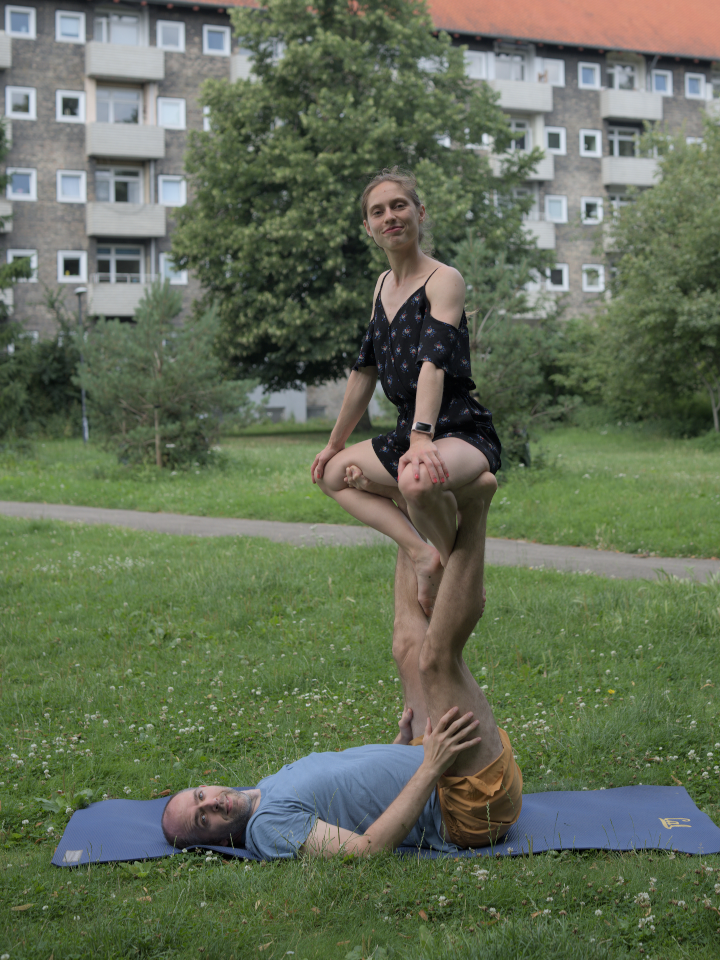
\includegraphics[width=45mm]{
    ./figs/dscf0013016.png
  }
          \end{minted}
        \end{minipage}
      };
      &
      \node[rectangle,thick,anchor=west,draw,minimum height=\height] (output) {
  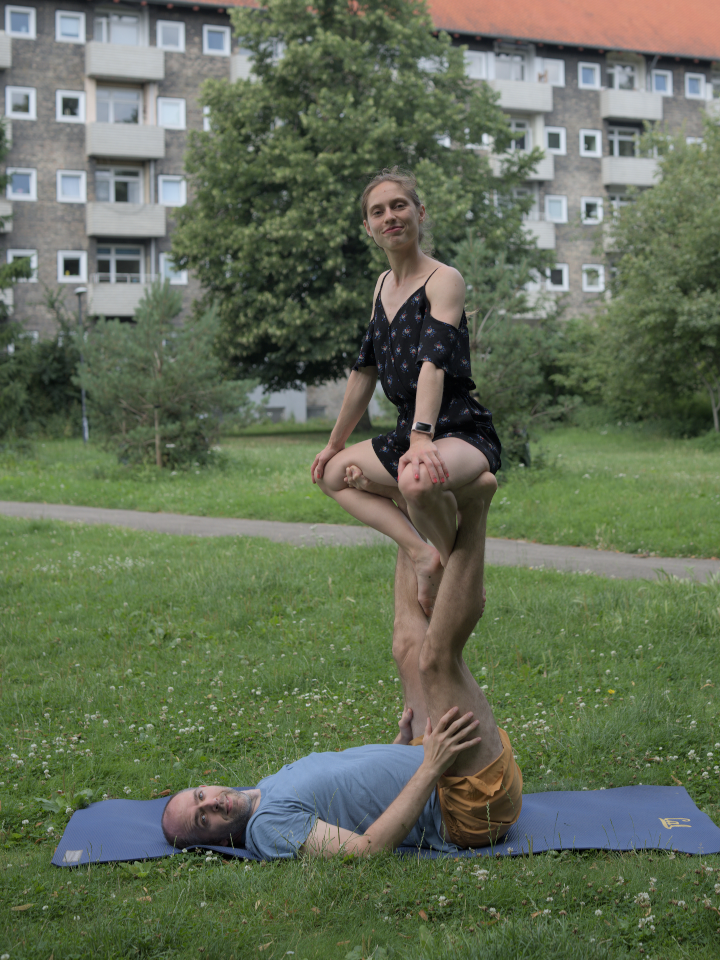
\includegraphics[width=45mm]{./figs/dscf0013016.png}
      };
      \\
    };
    
    \draw[dedge] (code)->(output);
  \end{tikzpicture}
\end{frame}

\subsection{Floats}
\begin{frame}[fragile]
  \frametitle{Floats}
  \vspace{3mm}
  When writing a report, you should expect your reader to follow the main track of the text. It should be possible to read it from beginning to end.
  
  \pause
  \vspace{5mm}
  But at times you may want to provide extra materials though figures and tables. These should not break the flow of the text.
  
  \pause
  \vspace{5mm}
  Instead, they should exists outside the flow of the text, and be referenced. The typesetting system should find space for them closeby, at a location where they don't break the flow.
  
  \pause
  \vspace{5mm}
  In short, they should \textcolor{purple}{\textsl{float}}.
\end{frame}

\subsubsection{Figures and Tables}
\begin{frame}[fragile]
  \frametitle{Floats \subpart{Figures and Tables}}
  \vspace{3mm}
  You define a figure like this:
  \begin{minted}{latex}
\begin{figure}[tbp]
  % contents goes here
  \caption{Description of figure}
  \label{fig:tag}
\end{figure}
  \end{minted}
  
  \pause
  \vspace{5mm}
  You define a table like this:
  \begin{minted}{latex}
\begin{table}[tbp]
  % contents goes here
  \caption{Description of table}
  \label{table:tag}
\end{table}
  \end{minted}
\end{frame}

\subsubsection{Positioning}
\begin{frame}[fragile]
  \frametitle{Floats \subpart{Positioning}}
  \vspace{0mm}
  \begin{minted}[escapeinside=||]{latex}
\begin{figure}[|\tikzmark{before}|tbp|\tikzmark{after}|]
  % contents goes here
  \caption{Description of figure}
  \label{fig:tag}
\end{figure}
  \end{minted}
  \pause
  \begin{tikzpicture}[remember picture]
    \tikzstyle{arrow} = [thick,->,>=stealth, draw=black]
    \tikzstyle{box} = [overlay,rectangle,thick,draw=black]
    
    \node[box,minimum width=7mm, minimum height=4mm] (box)
      at ([yshift= 1.1mm] $(pic cs:before)!0.5!(pic cs:after)$) {};
    
    \node[overlay,anchor=west] (label)
      at ([xshift=6mm] box.east) {What about this?};
    
    \draw[overlay, arrow, thick] (label) -- (box);
  \end{tikzpicture}
  
  \pause
  \vspace{-1mm}
  These are the positioning instructions. It instructs \LaTeX\ where it is allowed to place the float. It supports the following codes:
  \begin{itemize}
    \item \say{\textcolor{purple}{\texttt{t}}} Float can be placed at the top of a page.
    \item \say{\textcolor{purple}{\texttt{b}}} Float can be placed at the bottom of a page.
    \item \say{\textcolor{purple}{\texttt{p}}} Float can be placed at a page with nothing but floats.
    \item \say{\textcolor{purple}{\texttt{h}}} Float should be placed \textsl{approximately here}.
    \item \say{\textcolor{purple}{\texttt{!}}} Override internal parameters that \LaTeX\ uses to determine \textsl{good} positions.
  \end{itemize}
  
  \pause
  \vspace{2mm}
  In general, avoid the latter two.
\end{frame}

\subsection{Footnotes}
\begin{frame}[fragile]
  \frametitle{Footnotes}
  \begin{tikzpicture}[remember picture,overlay]
    \newcommand{\height}[0]{24mm}
    \newcommand{\dist}[0]{5mm}
    
    \tikzstyle{dedge} = [thick,->,>=stealth,draw=black]
    
    \node[rectangle,thick,anchor=east,draw,minimum height=\height] (code) at ([xshift=-\dist]current page.center) {
      \begin{minipage}{6cm}
        \begin{minted}{latex}
Text\footnote{Short
detailing.}.
        \end{minted}
      \end{minipage}
    };
    
    \node[rectangle,thick,anchor=west,draw,minimum height=\height] (output) at ([xshift=\dist]current page.center) {
      \begin{minipage}{6cm}
        Text\footnote{Short
        detaining.}.
      \end{minipage}
    };
    
    \draw[dedge] (code)->(output);
  \end{tikzpicture}
\end{frame}

\subsection{Margin Paragraphs}
\begin{frame}[fragile]
  \frametitle{Margin Paragraphs}
  \vspace{3mm}
  Margin paragraphs works in much the same way as footnotes.
  
  \vspace{5mm}
  However, they are (i) not numbered, and (ii) appear in the outer margin.
  
  \vspace{5mm}
  Instead of the \commandname{\textbackslash footnote} command you use \commandname{\textbackslash marginpar} (and make sure that the \packagename{marginnote} package is included).
  
  \begin{tikzpicture}[remember picture,overlay]
    \node[anchor=south] () at ([yshift=-42mm]current page.south) {
      \includeBitmap{marginpar.png}{14cm}
    };
  \end{tikzpicture}
\end{frame}

\subsection{Code Inclusion}
\begin{frame}[fragile]
  \frametitle{Code Inclusion}
  \vspace{3mm}
  There is a number of packages for including code. In this presentation we will look at \packagename{minted}.
  
  \vspace{5mm}
  The \packagename{minted} package support a long list of file format, and even things like shell interactions.
  
  \vspace{5mm}
  It also support various forms of highlights and line numbering.
\end{frame}

\subsubsection{Inline}
\begin{frame}[fragile]
  \frametitle{Code Inclusion \subpart{Inline}}
  \begin{tikzpicture}[remember picture,overlay]
    \newcommand{\height}[0]{24mm}
    \newcommand{\dist}[0]{5mm}
    
    \tikzstyle{dedge} = [thick,->,>=stealth,draw=black]
    
    \node[rectangle,thick,anchor=east,draw,minimum height=\height] (code) at ([xshift=-\dist]current page.center) {
      \begin{minipage}{6cm}
        \begin{minted}{latex}
The formatting of a function
call in rust looks like this:
\mintinline{rust}{fun(1+1)}.
        \end{minted}
      \end{minipage}
    };
    
    \node[rectangle,thick,anchor=west,draw,minimum height=\height] (output) at ([xshift=\dist]current page.center) {
      \begin{minipage}{6cm}
The formatting of a function
call in rust looks like this:
\mintinline{rust}{fun(1+1)}.
      \end{minipage}
    };
    
    \draw[dedge] (code)->(output);
  \end{tikzpicture}
\end{frame}

\subsubsection{Environment}
\begin{frame}[fragile]
  \frametitle{Code Inclusion \subpart{Environment}}
  \begin{tikzpicture}[remember picture,overlay]
    \newcommand{\height}[0]{44mm}
    \newcommand{\dist}[0]{5mm}
    
    \tikzstyle{dedge} = [thick,->,>=stealth,draw=black]
    
    \begin{scope}[scale=0.7,transform shape]
      \node[rectangle,thick,anchor=east,draw,minimum height=\height,minimum width=8cm,align=left] (code) at ([xshift=-\dist]current page.center) {
        \begin{minipage}{8cm}
          \inputminted[]{latex}{../src/code_inclusion/minted_inclusion.tex}
        \end{minipage}
      };
    \end{scope}
    
    \begin{scope}[scale=0.7,transform shape]
      \node[rectangle,thick,anchor=west,draw,minimum height=\height,minimum width=8cm,align=left] (output) at ([xshift=\dist]current page.center) {
        \begin{minipage}{8cm}
          The code could look like this:

\begin{minted}{elixir}
doubles =
  [1,2,3,4]
  |> Enum.map(fn value -> value*2 end)
\end{minted}

And that's not too bad, right?

        \end{minipage}
      };
    \end{scope}
    
    \draw[dedge] (code)->(output);
  \end{tikzpicture}
\end{frame}

\subsection{Mathematics}
\begin{frame}[fragile]
  \frametitle{Mathematics}
  \vspace{3mm}
  One of the things \LaTeX\ is know for is its ability to typeset mathematical expressions.
  
  \vspace{5mm}
  At first, it can be quite daunting to remember the syntax and code for all the different constructs.
  
  \vspace{5mm}
  But the reality is that there is a system behind the madness, and the set of constructs you are going to be using on a daily basis is very small and easily remembered.
  
  \vspace{5mm}
  For instance, the command for producing a fraction is called \commandname{\textbackslash frac} and takes two parameters: First a nominator, and then a denominator. The \commandname{\textbackslash sqrt} command produces a square root symbol and takes one parameter.
  
  \vspace{5mm}
  And the web is littered with tables containing codes for Greek letters and all kinds of weird symbols. Just do an image search.
\end{frame}

\subsubsection{Inline}
\begin{frame}[fragile]
  \frametitle{Mathematics \subpart{Inline}}
  \begin{tikzpicture}[remember picture,overlay]
    \newcommand{\height}[0]{24mm}
    \newcommand{\dist}[0]{5mm}
    
    \tikzstyle{dedge} = [thick,->,>=stealth,draw=black]
    
    \node[rectangle,thick,anchor=east,draw,minimum height=\height] (code) at ([xshift=-\dist]current page.center) {
      \begin{minipage}{6cm}
        \begin{minted}{latex}
The Pythagorean theorem
states that $a^2+b^2 = c^2$,
but can also be expressed as
$c = \sqrt{a^2+b^2}$.
        \end{minted}
      \end{minipage}
    };
    
    \node[rectangle,thick,anchor=west,draw,minimum height=\height] (output) at ([xshift=\dist]current page.center) {
      \begin{minipage}{6cm}
        The Pythagorean theorem states that $a^2+b^2 = c^2$, but can also be expressed as $c = \sqrt{a^2+b^2}$.
      \end{minipage}
    };
    
    \draw[dedge] (code)->(output);
  \end{tikzpicture}
\end{frame}

\subsubsection{Equations}
\begin{frame}[fragile]
  \frametitle{Mathematics \subpart{Equations}}
  \begin{tikzpicture}[remember picture,overlay]
    \newcommand{\height}[0]{24mm}
    \newcommand{\dist}[0]{5mm}
    
    \tikzstyle{dedge} = [thick,->,>=stealth,draw=black]
    
    \node[rectangle,thick,anchor=east,draw,minimum height=\height] (code) at ([xshift=-\dist]current page.center) {
      \begin{minipage}{6cm}
        \begin{minted}[fontsize=\footnotesize]{latex}
\begin{align*}
  a^2 &= b^2 + b^2 \Leftrightarrow \\
  a   &= \sqrt{b^2 + b^2}
\end{align*}
        \end{minted}
      \end{minipage}
    };
    
    \node[rectangle,thick,anchor=west,draw,minimum height=\height] (output) at ([xshift=\dist]current page.center) {
      \begin{minipage}{6cm}
\begin{align*}
  a^2 &= b^2 + b^2 \Leftrightarrow \\
  a   &= \sqrt{b^2 + b^2}
\end{align*}
      \end{minipage}
    };
    
    \draw[dedge] (code)->(output);
  \end{tikzpicture}
\end{frame}

\subsubsection{Equation References}
\begin{frame}[fragile]
  \frametitle{Mathematics \subpart{Equation References}}
  \begin{tikzpicture}[remember picture,overlay]
    \newcommand{\height}[0]{36mm}
    \newcommand{\dist}[0]{5mm}
    
    \tikzstyle{dedge} = [thick,->,>=stealth,draw=black]
    
    \node[rectangle,thick,anchor=east,draw,minimum height=\height] (code) at ([xshift=-\dist]current page.center) {
      \begin{minipage}{6.5cm}
        \begin{minted}[fontsize=\footnotesize]{latex}
\begin{align}
  \label{pyth1}
  a^2 &= b^2 + b^2 \Leftrightarrow \\
  \label{pyth2}
  a   &= \sqrt{b^2 + b^2}
\end{align}
Pythagoras can be expressed as
either of equations \ref{pyth1}
or \ref{pyth2}.
        \end{minted}
      \end{minipage}
    };
    
    \node[rectangle,thick,anchor=west,draw,minimum height=\height] (output) at ([xshift=\dist]current page.center) {
      \begin{minipage}{6.5cm}
\begin{align}
  \label{pyth1}
  a^2 &= b^2 + b^2 \Leftrightarrow \\
  \label{pyth2}
  a   &= \sqrt{b^2 + b^2}
\end{align}
Pythagoras can be expressed as
either of equations \ref{pyth1}
or \ref{pyth2}.
      \end{minipage}
    };
    
    \draw[dedge] (code)->(output);
  \end{tikzpicture}
\end{frame}

\subsubsection{Raising and Lowering Text}
\begin{frame}[fragile]
  \frametitle{Mathematics \subpart{Raising and Lowering Text}}
  \begin{tikzpicture}[remember picture,overlay]
    \newcommand{\height}[0]{24mm}
    \newcommand{\dist}[0]{5mm}
    
    \tikzstyle{dedge} = [thick,->,>=stealth,draw=black]
    
    \node[rectangle,thick,anchor=east,draw,minimum height=\height] (code) at ([xshift=-\dist]current page.center) {
      \begin{minipage}{6cm}
        \begin{minted}[fontsize=\footnotesize]{latex}
Water is $H_2O$.

$H_{20}$ is not a thing.

The square of three is $3^2$.
        \end{minted}
      \end{minipage}
    };
    
    \node[rectangle,thick,anchor=west,draw,minimum height=\height] (output) at ([xshift=\dist]current page.center) {
      \begin{minipage}{6cm}
Water is $H_2O$.

$H_{20}$ is not a thing.

The square of three is $3^2$.
      \end{minipage}
    };
    
    \draw[dedge] (code)->(output);
  \end{tikzpicture}
\end{frame}

\subsection{URLs}
\begin{frame}[fragile]
  \frametitle{URLs}
  \vspace{3mm}
  \begin{tikzpicture}[remember picture,overlay]
    \newcommand{\height}[0]{36mm}
    \newcommand{\dist}[0]{5mm}
    
    \tikzstyle{dedge} = [thick,->,>=stealth,draw=black]
    
    \node[rectangle,thick,anchor=east,draw,minimum height=\height] (code) at ([xshift=-\dist]current page.center) {
      \begin{minipage}{6cm}
        \begin{minted}[fontsize=\scriptsize]{latex}
Search at
\textcolor{blue}{
  \texttt{https://search.brave.com}
}

Search at
\url{https://search.brave.com}

Search at
\href{https://search.brave.com}{Brave}
        \end{minted}
      \end{minipage}
    };
    
    \node[rectangle,thick,anchor=west,draw,minimum height=\height] (output) at ([xshift=\dist]current page.center) {
      \scriptsize
      \begin{minipage}{6cm}
Search at
\textcolor{blue}{https://search.brave.com}

\vspace{3mm}
Search at
\url{https://search.brave.com}

\vspace{3mm}
Search at
\href{https://search.brave.com}{Brave}
      \end{minipage}
    };
    
    \draw[dedge] (code)->(output);
  \end{tikzpicture}
\end{frame}

\subsection{Nooks and Crannies}
\begin{frame}[fragile]
  \frametitle{Nooks and Crannies}
  \vspace{3mm}
  The \commandname{\textbackslash ldots} can be used to add three periods \ldots
  
  \vspace{5mm}
  Just as the \commandname{\textbackslash LaTeX} command, it will eat any following space. If this is not what you want, then you have to escape the following space with a backslash.
  
  \vspace{5mm}
  The \envname{center} environment and a \commandname{\textbackslash centering} command can be used to center elements.
\end{frame}

% background color post
}

%%%%%%%%%%%%%%%%%%%%%%%%%%%%%%%%%%%%%%%%%%%%%%%%%%%%%%%%%%%%%%%
%%%%%%%%%%%%%%%%%%%%%%%%%%%%%%%%%%%%%%%%%% Auto-Generated Lists

% background color pre
{
\setbeamercolor{background canvas}{bg=lists}
\renewcommand{\bgcolor}{lists}

\section{Auto-Generated Lists}
\begin{frame}
  \vspace{25mm}
  \begin{center}
    \Huge{Part 4:\\Auto-Generated Lists}
  \end{center}
\end{frame}

\subsection{Table of Contents}
\begin{frame}[fragile]
  \frametitle{Table of Contents}
  \vspace{3mm}
  
  When constructing the table of contents (aka ToC), we can decide how deep we want it to follow into the documents section tree.
  
  \vspace{5mm}
  If we want to include subsections, then we set the \texttt{tocdepth} counter to 2:
  \begin{minted}[gobble=0]{latex}
\setcounter{tocdepth}{2}
  \end{minted}
  
  \vspace{5mm}
  Alternatively, we can omit this.
  
  \pause
  \vspace{5mm}
  The ToC itself can be placed using this command:
  \begin{minted}[gobble=0]{latex}
\tableofcontents
  \end{minted}
  
  \pause
  \vspace{5mm}
  \textbf{Note:} All of this goes into the front matter of the document.
\end{frame}

\subsection{List of Figures and Tables}
\begin{frame}[fragile]
  \frametitle{List of Figures and Tables}
  \vspace{7mm}
  A list of figures can be inserted using the command:
  \begin{minted}[gobble=0]{latex}
\listoffigures
  \end{minted}
  
  \vspace{7mm}
  A list of tables can be inserted using the command:
  \begin{minted}[gobble=0]{latex}
\listoftables
  \end{minted}
\end{frame}

\subsection{Bibliography}
\begin{frame}[fragile]
  \frametitle{Bibliography}
  \vspace{3mm}
  When writing, we need to give and to take credit for the individual parts that make up our work.
  \begin{itemize}
    \item We build on what others have accomplished, and give them credit for their work.
    \item We come up with new insights, and take credit for those.
  \end{itemize}
  
  \pause
  \vspace{5mm}
  In order to give credit to some work, we \textsl{cite} it.
  
  \pause
  \vspace{5mm}
  \LaTeX\ has an extensive framework for working with such citations.
\end{frame}

\subsubsection{Database Population}
\begin{frame}[fragile]
  \frametitle{Bibliography \subpart{Database Population}}
  \vspace{3mm}
  
  \begin{tikzpicture}[remember picture,overlay]
    \node[anchor=north] () at ([yshift=-0.5cm]current page.north) {\only<1>{\includeBitmap{acmpaper1.png}{13cm}}\only<2>{\includeBitmap{acmpaper2.png}{13cm}}};
  \end{tikzpicture}
\end{frame}

\subsubsection{Database}
\begin{frame}[fragile]
  \frametitle{Bibliography \subpart{Database}}
  \vspace{7mm}
  \tikzmark{mark}
  \begin{minted}[gobble=0,breaklines,fontsize=\tiny]{bibtex}
@inproceedings{10.1145/1098918.1098925,
  author = {Tolle, Gilman and Polastre, Joseph and Szewczyk, Robert and Culler, David and Turner, Neil and Tu, Kevin and Burgess, Stephen and Dawson, Todd and Buonadonna, Phil and Gay, David and Hong, Wei},
  title = {A macroscope in the redwoods},
  year = {2005},
  isbn = {159593054X},
  publisher = {Association for Computing Machinery},
  address = {New York, NY, USA},
  url = {https://doi.org/10.1145/1098918.1098925},
  doi = {10.1145/1098918.1098925},
  abstract = {The wireless sensor network "macroscope" offers the potential to advance science by enabling dense temporal and spatial monitoring of large physical volumes. This paper presents a case study of a wireless sensor network that recorded 44 days in the life of a 70-meter tall redwood tree, at a density of every 5 minutes in time and every 2 meters in space. Each node measured air temperature, relative humidity, and photosynthetically active solar radiation. The network captured a detailed picture of the complex spatial variation and temporal dynamics of the microclimate surrounding a coastal redwood tree. This paper describes the deployed network and then employs a multi-dimensional analysis methodology to reveal trends and gradients in this large and previously-unobtainable dataset. An analysis of system performance data is then performed, suggesting lessons for future deployments.},
  booktitle = {Proceedings of the 3rd International Conference on Embedded Networked Sensor Systems},
  pages = {51–63},
  numpages = {13},
  keywords = {wireless sensor networks, microclimate monitoring, macroscope, application analysis},
  location = {San Diego, California, USA},
  series = {SenSys '05}
}
  \end{minted}
  \pause
  \begin{tikzpicture}[remember picture]
    \tikzstyle{arrow} = [thick,->,>=stealth, draw=black]
    \tikzstyle{box} = [overlay,rectangle,thick,draw=black]
    
    \node[box,minimum width=27mm, minimum height=4mm] (box)
      at ([xshift=29.5mm,yshift=-2.75mm] $(pic cs:mark)$) {};
    
    \node[overlay,anchor=south] (label)
      at ([yshift=4mm] box.north) {Remember this!};
    
    \draw[overlay, arrow, thick] (label) -- (box);
  \end{tikzpicture}
\end{frame}

\subsubsection{Citation and Bibliography Generation}
\begin{frame}[fragile]
  \frametitle{Bibliography \subpart{Citation and Bibliography Generation}}
  \vspace{-2mm}
  Assuming that you have that database stored in \filename{references.bib}, put the following in your preample:
  \begin{minted}[gobble=0]{latex}
\usepackage[
  backend=biber,
]{biblatex}
\addbibresource{references.bib}
  \end{minted}
  
  \pause
  \vspace{3mm}
  Now you can start citing your statements:
  \begin{minted}[gobble=0]{latex}
Some profound statement\cite{10.1145/1098918.1098925}.
  \end{minted}
  
  \pause
  \vspace{3mm}
  We can then add the bibliography in the back matter:
  \begin{minted}[gobble=0]{latex}
\printbibliography
  \end{minted}
  
  \pause
  \vspace{3mm}
  In between the first and the later runs of \LaTeX, make sure to run the following command:
  \begin{minted}[gobble=0]{latex}
biber document.bcf
  \end{minted}
\end{frame}

\subsection{Index}
\begin{frame}[fragile]
  \frametitle{Index}
  \vspace{3mm}
  At its core, an index allows us to look up a term and get a set of pages relevant for that term.
  
  \vspace{4mm}
  To tag a position for inclusion in the index under a specific term, use the command:
  \begin{minted}[gobble=0]{latex}
\index{Term}
  \end{minted}
  
  \pause
  \vspace{4mm}
  At the back matter of your document, then add:
  \begin{minted}[gobble=0]{latex}
\printindex
  \end{minted}
  
  \pause
  \vspace{4mm}
  In between the first and the later runs of \LaTeX, make sure to run the following command:
  \begin{minted}[gobble=0]{shell}
makeindex document.idx
  \end{minted}
  
  \vspace{4mm}
  It will generate your index.
\end{frame}

% background color post
}

%%%%%%%%%%%%%%%%%%%%%%%%%%%%%%%%%%%%%%%%%%%%%%%%%%%%%%%%%%%%%%%
%%%%%%%%%%%%%%%%%%%%%%%%%%%%%%%%%%%%%%%%%%% Dealing with Errors

% background color pre
{
\setbeamercolor{background canvas}{bg=errors}
\renewcommand{\bgcolor}{errors}

\section{Dealing with Errors}
\begin{frame}
  \vspace{25mm}
  \begin{center}
    \Huge{Part 5:\\Dealing with Errors}
  \end{center}
\end{frame}

\subsection{Locating the Error}
\begin{frame}[fragile]
  \frametitle{Locating the Error}
  \vspace{3mm}
  Unfortunately, \LaTeX\ errors are notorious for being hard to reason about.
  
  \pause
  \vspace{5mm}
  Often, the line number does not reflect the actual line in the source file.
  
  \pause
  \vspace{5mm}
  Because of this, I often build the document.
  
  \pause
  \vspace{5mm}
  If in doubt, use binary search by commenting out large blocks of code to locate the issue.
\end{frame}

\subsection{Googling the Error}
\begin{frame}[fragile]
  \frametitle{Googling the Error}
  \vspace{3mm}
  Most errors are easily googleable, and will yield hits on sites like StackOverflow.
  
  \pause
  \vspace{5mm}
  In order to get good results, you should:
  \begin{itemize}
    \item Carefully consider which part to copy paste in. These errors can be verbose.
    \item Consider the type of error.
    \item Try to figure out what could cause such an error, and figure out whether these conditions apply to you.
    \item Don't be afraid to take an extra step down the rabbit hole.
  \end{itemize}
\end{frame}

% background color post
}

%%%%%%%%%%%%%%%%%%%%%%%%%%%%%%%%%%%%%%%%%%%%%%%%%%%%%%%%%%%%%%%
%%%%%%%%%%%%%%%%%%%%%%%%%%%%%%%%%%%%%%%%%%%%%%%%%%%%% Templates

% background color pre
{
\setbeamercolor{background canvas}{bg=templates}
\renewcommand{\bgcolor}{templates}

\section{Resources}
\begin{frame}
  \vspace{25mm}
  \begin{center}
    \Huge{Part 6:\\Resources}
  \end{center}
\end{frame}

\subsection{General Resources}
\begin{frame}[fragile]
  \frametitle{General Resources}
  \vspace{3mm}
  Wide resources:
  \begin{itemize}
    \item WikiBooks LaTeX: \url{https://en.wikibooks.org/wiki/LaTeX}
    \item Overleaf Learn: \url{https://www.overleaf.com/learn}
  \end{itemize}
  
  \pause
  \vspace{5mm}
  Code generators:
  \begin{itemize}
    \item Table generator: \url{https://www.tablesgenerator.com/latex_tables}
    \item Equation editor: \url{https://latexeditor.lagrida.com}
  \end{itemize}
  
  \pause
  \vspace{5mm}
  Misc:
  \begin{itemize}
    \item \TikZ: \url{https://tikz.dev}
  \end{itemize}
\end{frame}

\subsection{Source}
\begin{frame}[fragile]
  \frametitle{Source}
  \vspace{3mm}
  The source code for these slides can be found here: \url{https://github.com/aslakjohansen/prosa-latex}
\end{frame}

\subsection{Templates}
\begin{frame}[fragile]
  \frametitle{Templates}
  \vspace{3mm}
  Report
  
  \vspace{5mm}
  Presentation
\end{frame}

% background color post
}

%%%%%%%%%%%%%%%%%%%%%%%%%%%%%%%%%%%%%%%%%%%%%%%%%%%%%%%%%%%%%%%
%%%%%%%%%%%%%%%%%%%%%%%%%%%%%%%%%%%%%%%%%%%%%%%%%%%%% Exercises

% background color pre
{
\setbeamercolor{background canvas}{bg=exercises}
\renewcommand{\bgcolor}{exercises}

\section{Exercises}
\begin{frame}
  \vspace{25mm}
  \begin{center}
    \Huge{Part 7:\\Exercises}
  \end{center}
\end{frame}

\subsection{Exercises}
\begin{frame}[fragile]
  \frametitle{Exercises}
  \vspace{3mm}
  \begin{enumerate}
    \descitem{New Project:} Create a new project (on Overleaf, GitHub or similar). Make sure that you have a report \LaTeX\ document that builds.
    \descitem{Tabular Data:} Find some tabular data, place it in a \texttt{tabular} environment, and make it look pretty.
    \descitem{Formula:} Pick any formula (e.g., the discrete fourier transformation), and express it though \LaTeX\ code.
    \descitem{Report:} Pick any old report, and port it to \LaTeX. The point is not to go through the whole report, but rather to get a feel of (i) the effort needed to port an old report, and (ii) the perceived typographical quality per effort.
  \end{enumerate}
\end{frame}

% background color post
}

